% Source: printed p. 447; PDF p. 456
đọc được thành một câu, nhưng không tương ứng với một hàm vì một người có thể không có con hoặc có nhiều hơn một người con. Ta gọi một olog mà mỗi mũi tên tương ứng với một hàm (lựa chọn duy nhất được đề xuất đến đây trong sách) là một \emph{olog mang tính hàm}. Yêu cầu olog mang tính hàm có cả ưu điểm lẫn nhược điểm. Ưu điểm chính là việc tạo ra một olog mang tính hàm đòi hỏi sự rõ ràng hơn về khái niệm, và điều này có lợi cho người tạo olog cũng như bất kỳ ai mà người ấy cố giải thích tình huống cho. Nhược điểm chính là việc tạo ra một olog mang tính hàm mất nhiều thời gian hơn, và olog chiếm nhiều chỗ hơn trên trang giấy.

Trong bối cảnh monad tập lũy thừa (xem Bài tập~7.3.2.3), một cấu xạ $f:X\to Y$ giữa các tập $X$ và $Y$, xem như đối tượng của $\operatorname{Kls}(\mathbb P)$, trở thành một quan hệ hai ngôi trên $X$ và $Y$ thay vì một hàm (xem Bài tập~7.3.3.5). Vì vậy, trong bối cảnh ấy, mũi tên ở~(7.14) trở nên hợp lệ. Một olog mà các mũi tên chỉ tương ứng với quan hệ hai ngôi thay vì hàm có thể được gọi là một \emph{olog quan hệ}.

\subsection{Monad trong cơ sở dữ liệu}
Mục này bàn về cách ghi dữ liệu khi có một monad. Ý tưởng khá đơn giản. Cho một lược đồ (phạm trù) $\mathcal C$, một thể hiện thông thường là một hàm tử $I:\mathcal C\to\Set$. Nhưng nếu $\top=(T,\eta,\mu)$ là một monad, thì một \emph{thể hiện Kleisli $\top$ trên $\mathcal C$} là một hàm tử $J:\mathcal C\to\operatorname{Kls}(\top)$. Hàm tử này gán cho mỗi đối tượng $c\in\Ob(\mathcal C)$ một tập $J(c)$, và cho mỗi mũi tên $f:c\to c'$ trong $\mathcal C$ một cấu xạ $J(f):J(c)\to J(c')$ trong $\operatorname{Kls}(\top)$. Điều này thể hiện thế nào dưới dạng bảng?

Nhắc lại rằng để biểu diễn một thể hiện cơ sở dữ liệu thông thường $I:\mathcal C\to\Set$, ta dùng dạng bảng, trong đó mỗi đối tượng $c\in\Ob(\mathcal C)$ được trình bày thành một bảng gồm một cột ID và một cột bổ sung ứng với mỗi mũi tên $f:c\to c'$ đi ra từ $c$. Các ô trong cột ID của bảng $c$ chứa các phần tử của tập $I(c)$, còn các ô trong cột $f$ chứa các phần tử của tập $I(c')$.

Biểu diễn một thể hiện cơ sở dữ liệu Kleisli $J:\mathcal C\to\operatorname{Kls}(\top)$ cũng tương tự; ta lại dùng dạng bảng, trong đó mỗi đối tượng $c\in\Ob(\mathcal C)$ được trình bày thành một bảng gồm một cột ID và một cột bổ sung ứng với mỗi mũi tên $f:c\to c'$ đi ra từ $c$. Các ô trong cột ID của bảng $c$ vẫn chứa các phần tử của tập $J(c)$; tuy nhiên, các ô trong cột $f$ không chứa các phần tử của $J(c')$, mà chứa các \emph{giá trị $T$ trong $J(c')$}, tức các phần tử của $T(J(c'))$.

\noindent\textit{Ví dụ 7.3.4.1.}\keepwithnext
Cho $\top=(T,\eta,\mu)$ là monad cho hàm bộ phận (xem Ví dụ~7.3.1.1). Với bất kỳ lược đồ $\mathcal C$, ta có thể biểu diễn một thể hiện Kleisli $\top$, $I:\mathcal C\to\operatorname{Kls}(\top)$, dưới dạng bảng. Với mỗi đối tượng $c\in\Ob(\mathcal C)$, ta có một tập các hàng $I(c)$; cho một cột $f:c\to c'$, áp dụng $f$ lên một hàng sẽ tạo ra một giá trị trong $I(c')$ hoặc không tạo ra giá trị nào; đây là bản chất của hàm bộ phận. Ta có thể ký hiệu sự vắng mặt của một giá trị bằng $\ctsevensmiley$.

% Source: printed p. 448; PDF p. 457
Xét lược đồ chỉ mục cho đồ thị
\[
\mathcal C:=\begin{tikzpicture}[>=Stealth,baseline=-.5ex,font=\scriptsize]
\draw(-.65,-.55)rectangle(3.65,1.05);
\node[circle,fill,inner sep=1.1pt,label=above:{\shortstack{Mũi tên\\Arrow}}](a)at(0,0){};
\node[circle,fill,inner sep=1.1pt,label=above:{\shortstack{Đỉnh\\Vertex}}](v)at(3,0){};
\draw[->](a)to[bend left=12]node[above]{$\mathrm{src}$}(v);\draw[->](a)to[bend right=12]node[below]{$\mathrm{tgt}$}(v);
\end{tikzpicture}
\]
Như đã bàn ở Mục~5.2.1.21, một thể hiện thông thường trên $\mathcal C$ biểu diễn một đồ thị:
\begin{center}
\begin{tikzpicture}[>=Stealth,font=\small,pt/.style={circle,fill,inner sep=1.1pt}]
\node at(-.9,0){$I:=$};\draw(-.45,-.75)rectangle(3.1,.75);
\node[pt,label=above:$v$](v)at(0,0){};\node[pt,label=above:$w$](w)at(1.3,0){};\node[pt,label=above:$x$](x)at(2.7,0){};
\draw[->](v)--node[above]{$f$}(w);\draw[->](w)to[bend left=35]node[above]{$g$}(x);\draw[->](w)to[bend right=35]node[below]{$h$}(x);
\end{tikzpicture}
\end{center}
\[
\begin{array}{|c||c|c|}\hline\multicolumn{3}{|c|}{\mathrm{Arrow}\ (I)}\\\hline\text{ID}&\mathrm{src}&\mathrm{tgt}\\\hline f&v&w\\\hline g&w&x\\\hline h&w&x\\\hline\end{array}\qquad
\begin{array}{|c||}\hline\mathrm{Vertex}\ (I)\\\hline\text{ID}\\\hline v\\\hline w\\\hline x\\\hline\end{array}
\]
Một thể hiện Kleisli $\top$ trên $\mathcal C$ biểu diễn những đồ thị trong đó cạnh có thể không có đỉnh nguồn, không có đỉnh đích, hoặc không có cả hai:
\begin{center}
\begin{tikzpicture}[>=Stealth,font=\small,pt/.style={circle,fill,inner sep=1.1pt}]
\node at(-.9,-.35){$J:=$};\draw(-.45,-1.45)rectangle(3.1,.75);
\node[pt,label=above:$v$](v)at(0,0){};\node[pt,label=above:$w$](w)at(1.3,0){};\node[pt,label=above:$x$](x)at(2.7,0){};
\draw[->](v)--node[above]{$f$}(w);\draw[->](w)to[bend left=35]node[above]{$g$}(x);\draw[->](w)to[bend right=35]node[below]{$h$}(x);
\draw[->](v)--node[left]{$i$}(0,-.85);\draw[->](1.5,-.85)--node[below]{$j$}(2.8,-.85);
\end{tikzpicture}
\end{center}
\[
\begin{array}{|c||c|c|}\hline\multicolumn{3}{|c|}{\mathrm{Arrow}\ (J)}\\\hline\text{ID}&\mathrm{src}&\mathrm{tgt}\\\hline f&v&w\\\hline g&w&x\\\hline h&w&x\\\hline i&v&\ctsevensmiley\\\hline j&\ctsevensmiley&\ctsevensmiley\\\hline\end{array}\qquad
\begin{array}{|c||}\hline\mathrm{Vertex}\ (J)\\\hline\text{ID}\\\hline v\\\hline w\\\hline x\\\hline\end{array}
\]
Bối cảnh của các bảng này là hàm bộ phận, nên ta không cần một tham chiếu cho $\ctsevensmiley$ trong bảng đỉnh. Về mặt toán học, cấu xạ $J(\mathrm{src}):J(\mathrm{Arrow})\to J(\mathrm{Vertex})$ trong $\operatorname{Kls}(\top)$ phải là một hàm $J(\mathrm{Arrow})\to J(\mathrm{Vertex})\sqcup\{\ctsevensmiley\}$, và đúng là như vậy.

\subsubsection*{7.3.4.2\quad Phân phối xác suất}
Cho $[0,1]\subseteq\mathbb R$ ký hiệu tập các số thực từ 0 đến 1. Cho $X$ là một tập và $p:X\to[0,1]$ là một hàm. Ta nói $p$ là một \emph{phân phối xác suất có giá hữu hạn trên $X$} nếu tồn tại một tập con hữu hạn $W\subseteq X$ sao cho
\stepcounter{equation}
\begin{equation}
\sum_{w\in W}p(w)=1,
\tag{7.15}
\end{equation}
% Source: printed p. 449; PDF p. 458
và $p(x)>0$ khi và chỉ khi $x\in W$. Chú ý rằng tập con $W$ là duy nhất nếu nó tồn tại; ta gọi nó là \emph{giá của $p$} và ký hiệu $\operatorname{Supp}(p)$.

Với bất kỳ tập $X$, cho $\operatorname{Dist}(X)$ ký hiệu tập các phân phối xác suất có giá hữu hạn trên $X$. Dễ kiểm tra rằng cho một hàm $f:X\to Y$, ta được một hàm $\operatorname{Dist}(f):\operatorname{Dist}(X)\to\operatorname{Dist}(Y)$ bởi:\ctsevennote{Nguyên bản viết ``$\operatorname{Dist}(f)(y)=\sum_{f(x)=y}p(x)$''. Nhưng $\operatorname{Dist}(f)$ nhận đầu vào là một phân phối $p$, và kết quả mới là hàm trên $Y$. Bản dịch bổ sung đối số $p$ để biểu thức có đúng kiểu và chỉ rõ phân phối đang được đẩy tới.}
\[
\operatorname{Dist}(f)(p)(y)=\sum_{f(x)=y}p(x).
\]
Vì vậy, ta có thể coi $\operatorname{Dist}:\Set\to\Set$ là một hàm tử, và thực ra là phần hàm tử của một monad. Đơn vị $\eta:X\to\operatorname{Dist}(X)$ của nó được cho bởi hàm delta Kronecker $x\mapsto\delta_x$, trong đó $\delta_x(x)=1$ và $\delta_x(x')=0$ với $x'\ne x$. Phép nhân $\mu:\operatorname{Dist}(\operatorname{Dist}(X))\to\operatorname{Dist}(X)$ được cho bởi tổng có trọng số: cho một phân phối xác suất có giá hữu hạn $w:\operatorname{Dist}(X)\to[0,1]$ và $x\in X$, đặt
\[
\mu(w)(x)=\sum_{p\in\operatorname{Supp}(w)}w(p)p(x).
\]

\noindent\textit{Ví dụ 7.3.4.3 (Chuỗi Markov).}\keepwithnext
Cho $\mathit{Loop}$ là lược đồ vòng lặp
\[
\mathit{Loop}:=\begin{tikzpicture}[>=Stealth,baseline=-.5ex]
\draw(-.55,-.55)rectangle(.55,1.15);\node[circle,fill,inner sep=1.1pt,label=right:$s$](s)at(0,0){};
\draw[->](s)to[loop above,min distance=8mm,looseness=6]node[left]{$f$}(s);
\end{tikzpicture}
\]
như trong Ví dụ~4.5.2.10. Một thể hiện $\operatorname{Dist}$ trên $\mathit{Loop}$ tương đương với một \emph{chuỗi Markov thuần nhất theo thời gian}. Cụ thể, một hàm tử $\delta:\mathit{Loop}\to\operatorname{Kls}(\operatorname{Dist})$ gán cho đối tượng duy nhất $s\in\Ob(\mathit{Loop})$ một tập $S=\delta(s)$, gọi là \emph{không gian trạng thái}, và cho $f:s\to s$ một hàm $\delta(f):S\to\operatorname{Dist}(S)$, gửi mỗi phần tử $x\in S$ đến một phân phối xác suất trên các phần tử của $S$. Chẳng hạn, bảng $\delta$ bên trái (có các trạng thái $\delta(s)=\{a,b,c,d\}$) tương ứng với ma trận Markov $M$ bên phải:
\stepcounter{equation}
\begin{equation}
\delta:=\begin{array}{|l||l|}\hline\multicolumn{2}{|c|}{s}\\\hline\text{ID}&f\\\hline
a&.5(a)+.5(b)\\\hline b&1(b)\\\hline c&.7(a)+.3(c)\\\hline d&.4(a)+.3(b)+.3(d)\\\hline\end{array}
\qquad M:=\begin{pmatrix}.5&.5&0&0\\0&1&0&0\\.7&0&.3&0\\.4&.3&0&.3\end{pmatrix}
\tag{7.16}
\end{equation}
Như ta có thể mong đợi, với bất kỳ số tự nhiên $n\in\mathbb N$, ánh xạ $f^n:S\to S$ trong $\operatorname{Kls}(\operatorname{Dist})$ tương ứng với ma trận $M^n$, gửi một phần tử $s\in S$ đến phân phối vị trí có khả năng của nó sau $n$ lần lặp ánh xạ chuyển trạng thái, $f^n(s)\in\operatorname{Dist}(S)$.

\noindent\textit{Ứng dụng 7.3.4.4.}\keepwithnext
Mỗi ngôi sao phát ra một phổ ánh sáng, có thể được hiểu là một phân phối trên phổ điện từ. Cho một vật thể $B$ trên Trái Đất, các phần khác nhau của $B$ hấp thụ bức xạ ở những mức khác nhau. Vì vậy $B$ cho một hàm từ phổ điện từ đến các phân phối mức hấp thụ năng lượng. Trong bối cảnh monad phân phối xác suất, ta có thể ghi dữ liệu trên lược đồ
\begin{center}
\begin{tikzpicture}[>=Stealth,font=\scriptsize,pt/.style={circle,fill,inner sep=1.1pt}]
\node[pt,label=above:{ngôi sao}](s)at(0,0){};\node[pt,label=above:{bước sóng}](w)at(3.6,0){};\node[pt,label=above:{năng lượng}](e)at(7.5,0){};
\draw[->](s)--node[above]{phát ra}(w);\draw[->](w)--node[above]{được $B$ hấp thụ}(e);
\end{tikzpicture}
\end{center}
% Source: printed p. 450; PDF p. 459
Công thức hợp thành cho phạm trù Kleisli đúng như mong muốn: ta gán cho mỗi ngôi sao tổng có trọng số của các mức hấp thụ năng lượng trên tập các bước sóng mà ngôi sao phát ra.
\hfill$\diamond\diamond$

\subsection{Monad và liên hợp}
Có một mối liên hệ chặt chẽ giữa monad và liên hợp: mỗi liên hợp tạo ra một monad, và mỗi monad xuất phát từ một liên hợp. Chẳng hạn, monad $\operatorname{List}$ (Ví dụ~7.3.2.2) xuất phát từ liên hợp tự do--quên giữa tập hợp và monoid
\[
\begin{tikzcd}[column sep=large]\Set\arrow[r,bend left=20,"F"]&\mathbf{Mon}\arrow[l,bend left=20,"U"]\end{tikzcd}
\]
(xem Mệnh đề~7.1.1.2). Nghĩa là, với bất kỳ tập $X$, monoid tự do trên $X$ là
\[
F(X)=(\operatorname{List}(X),[\,],{+}{+}),
\]
và tập nền của monoid ấy là $U(F(X))=\operatorname{List}(X)$. Vậy hàm tử $\operatorname{List}$ được cho bởi $U\circ F:\Set\to\Set$. Nhưng một monad không chỉ là một hàm tử; nó gồm một ánh xạ đơn vị $\eta$ và một ánh xạ nhân $\mu$ (xem Định nghĩa~7.3.2.1). May thay, đơn vị $\eta$ và phép nhân $\mu$ cũng xuất hiện từ liên hợp. Trước hết, ta bàn về đơn vị và đối đơn vị của một liên hợp.

\noindent\textbf{Định nghĩa 7.3.5.1.}\keepwithnext
Cho $\mathcal C$ và $\mathcal D$ là các phạm trù, cho $L:\mathcal C\to\mathcal D$ và $R:\mathcal D\to\mathcal C$ là các hàm tử với đẳng cấu liên hợp
\[
\alpha_{c,d}:\Hom_{\mathcal D}(L(c),d)\xrightarrow{\cong}\Hom_{\mathcal C}(c,R(d))
\]
với mọi đối tượng $c\in\Ob(\mathcal C)$ và $d\in\Ob(\mathcal D)$ (xem Định nghĩa~7.1.1.1). \emph{Đơn vị $\eta:\id_{\mathcal C}\to R\circ L$} (tương ứng, \emph{đối đơn vị $\epsilon:L\circ R\to\id_{\mathcal D}$}) của liên hợp là một biến đổi tự nhiên được định nghĩa như sau.

Cho một đối tượng $c\in\Ob(\mathcal C)$, ta áp dụng $\alpha$ lên $\id_{L(c)}:L(c)\to L(c)$ để được thành phần tại $c$ của $\eta$,
\[
\eta_c:c\longrightarrow R\circ L(c).
\]
Tương tự, cho một đối tượng $d\in\Ob(\mathcal D)$, ta áp dụng $\alpha^{-1}$ lên $\id_{R(d)}:R(d)\to R(d)$ để được thành phần tại $d$,
\[
\epsilon_d:L\circ R(d)\longrightarrow d.
\]
Có thể kiểm tra rằng các thành phần này là tự nhiên.

Sau đây ta sẽ thấy cách dùng đơn vị và đối đơn vị của bất kỳ liên hợp nào để tạo một monad. Trước hết, ta đi qua quá trình ấy trong Ví dụ~7.3.5.2.

% Source: printed p. 451; PDF p. 460
\noindent\textit{Ví dụ 7.3.5.2.}\keepwithnext
Xét liên hợp $\Set\underset{U}{\overset{F}{\rightleftarrows}}\mathbf{Mon}$ giữa tập hợp và monoid. Cho $T=U\circ F:\Set\to\Set$; đây sẽ là phần hàm tử của monad, và ta đã thấy $T=\operatorname{List}$. Đơn vị của liên hợp $\eta:\id_{\Set}\to U\circ F$ chính là đơn vị của monad: với bất kỳ tập $X\in\Ob(\Set)$, thành phần $\eta_X:X\to\operatorname{List}(X)$ là hàm đưa $x\in X$ đến danh sách một phần tử $[x]\in\operatorname{List}(X)$. Monad còn có một ánh xạ nhân $\mu_X:T(T(X))\to T(X)$, chính là nối một danh sách của các danh sách. Hàm này xuất hiện qua đối đơn vị $\epsilon$ như sau:
\[
T\circ T=U\circ F\circ U\circ F\xrightarrow{\id_U\diamond\epsilon\diamond\id_F}U\circ F=T.
\]
Quy trình tổng quát để rút ra một monad từ một liên hợp tương tự quá trình ở Ví dụ~7.3.5.2. Cho bất kỳ liên hợp
\[
\begin{tikzcd}[column sep=large]\mathcal C\arrow[r,bend left=20,"L"]&\mathcal D\arrow[l,bend left=20,"R"]\end{tikzcd},
\]
ta định nghĩa $\top=R\circ L:\mathcal C\to\mathcal C$, định nghĩa $\eta:\id_{\mathcal C}\to\top$ là đơn vị của liên hợp (như ở Định nghĩa~7.3.5.1), và định nghĩa $\mu:\top\circ\top\to\top$ là biến đổi tự nhiên $\id_R\diamond\epsilon\diamond\id_L:RLRL\to RL$, thu được bằng cách áp dụng đối đơn vị $\epsilon:LR\to\id_{\mathcal D}$.

Quy trình này tạo ra monad trên các phạm trù tùy ý $\mathcal C$, trong khi định nghĩa monad (Định nghĩa~7.3.2.1) chỉ xét trường hợp $\mathcal C=\Set$. Tuy nhiên, có thể tổng quát hóa Định nghĩa~7.3.2.1 sang các phạm trù tùy ý $\mathcal C$ chỉ bằng cách thay mọi chỗ xuất hiện của chuỗi $\Set$ bằng chuỗi $\mathcal C$. Tương tự, định nghĩa phạm trù Kleisli (Định nghĩa~7.3.3.1) chỉ xét trường hợp $\mathcal C=\Set$, nhưng việc tổng quát hóa sang các phạm trù tùy ý $\mathcal C$ cũng trực tiếp như vậy.

\noindent\textit{Ví dụ 7.3.5.3.}\keepwithnext
Cho $A\in\Ob(\Set)$ là một tập, và nhắc lại liên hợp currying
\[
\begin{tikzcd}[column sep=huge]\Set\arrow[r,bend left=20,"X\mapsto X\times A"]&\Set\arrow[l,bend left=20,"Y\mapsto Y^A"]\end{tikzcd},
\]
đã được bàn ngắn gọn ở Ví dụ~7.1.1.8. Trong lý thuyết ngôn ngữ lập trình, monad tương ứng $\operatorname{St}_A$ thường được gọi là \emph{monad trạng thái kiểu $A$}. Cho một tập $X$, ta có $\operatorname{St}_A(X)=(A\times X)^A$.

Trong phạm trù Kleisli $\operatorname{Kls}(\operatorname{St}_A)$, một cấu xạ từ $X$ đến $Y$ là một hàm có dạng $X\to(A\times Y)^A$, nhưng có thể chuyển qua currying thành một hàm $A\times X\to A\times Y$.

Như đã bàn ở Nhận xét~7.3.3.9, monad này liên quan đến việc giữ một biến trạng thái nội bộ kiểu $A$. Với monad trạng thái $\operatorname{St}_A$, mỗi cấu xạ viết là $X\to Y$, khi được xem như một hàm, nhận đầu vào không chỉ là một phần tử của $X$ mà còn cả trạng thái hiện tại $a\in A$, và tạo đầu ra không chỉ là một phần tử của $Y$ mà còn cả một trạng thái đã cập nhật.
% Source: printed p. 452; PDF p. 461
Các nhà khoa học máy tính nghiên cứu lý thuyết ngôn ngữ lập trình thấy monad rất hữu ích (Moggi~[33]). Theo một cách khá tương tự, monad trên $\Set$ có thể hữu ích trong cơ sở dữ liệu (xem Mục~7.3.4). Một cách khác, hoàn toàn khác biệt, để dùng monad trong cơ sở dữ liệu là dùng một ánh xạ giữa các lược đồ để tạo trong mỗi lược đồ một mô hình nội bộ của lược đồ kia. Nghĩa là, với bất kỳ hàm tử $F:\mathcal C\to\mathcal D$, tức một ánh xạ lược đồ cơ sở dữ liệu, liên hợp $(\Sigma_F,\Delta_F)$ tạo một monad trên $\mathcal C\text{--}\Set$, còn liên hợp $(\Delta_F,\Pi_F)$ tạo một monad trên $\mathcal D\text{--}\Set$. Nếu diễn giải monad $\operatorname{List}$ là tạo trong $\Set$ một mô hình nội bộ của phạm trù $\mathbf{Mon}$ các monoid, ta cũng có thể diễn giải những monad trên $\mathcal C\text{--}\Set$ và $\mathcal D\text{--}\Set$ là tạo các mô hình nội bộ của mỗi phạm trù bên trong phạm trù kia.

\section{Operad}
Mục này giới thiệu ngắn gọn operad, những tổng quát hóa của phạm trù. Chúng thường hữu ích để nói về tính tự đồng dạng của cấu trúc. Chẳng hạn, ta dùng operad để mô hình hóa các tác nhân được tạo từ những tác nhân nhỏ hơn, hoặc các vật liệu được tạo từ những vật liệu nhỏ hơn. Mối liên hệ với tính tự đồng dạng này không thực sự nằm sẵn trong định nghĩa, nhưng thường xuất hiện khi suy nghĩ về nhiều operad dùng trong thực tế.

Tôi xin bắt đầu bằng một lời cảnh báo.

\noindent\textit{Cảnh báo 7.4.0.4.}\keepwithnext
Cách tôi dùng từ \emph{operad} không hoàn toàn theo chuẩn và khác với cách dùng phổ biến. Thuật ngữ thông dụng hơn cho thứ tôi gọi là một operad là \emph{operad có màu} hoặc \emph{đa phạm trù đối xứng}. Theo cách dùng cổ điển, một operad là một đa phạm trù có một đối tượng, còn một operad có màu là một đa phạm trù có thể có nhiều đối tượng (mỗi đối tượng ứng với một ``màu''). Từ \emph{đa phạm trù} xuất phát từ việc các cấu xạ trong đa phạm trù có nhiều đối tượng miền, thay vì một. Một lý do tôi không thích dùng từ đa phạm trù là bản thân đa phạm trù không thực sự có gì ``đa'', chỉ các cấu xạ của nó mới có. Hơn nữa, tôi không thấy đủ lý do để phân biệt, khi từ đa phạm trù có vẻ khá cồng kềnh còn từ operad có vẻ khá gọn. Tôi hy vọng việc rời khỏi thuật ngữ chuẩn này không gây nhầm lẫn.

Phần giới thiệu operad này khá ngắn; xem Leinster~[25] để có một trình bày xuất sắc. Operad còn liên quan đến phạm trù monoidal, một chủ đề không được trình bày sâu trong sách này, nhưng đã được nhắc ngắn gọn khi bàn về làm giàu tôpô ở Ví dụ~5.2.3.3. Nhiều operad dưới đây thực chất là những phạm trù monoidal dưới một hình thức khác.

\subsection{Định nghĩa và các ví dụ cổ điển}
Một operad giống một phạm trù ở chỗ nó có đối tượng, cấu xạ và một công thức hợp thành, đồng thời tuân theo luật đồng nhất và luật kết hợp. Khác biệt là mỗi cấu xạ $f$ trong một operad có thể có nhiều đầu vào (và một đầu ra):
% Source: printed p. 453; PDF p. 462
\begin{center}
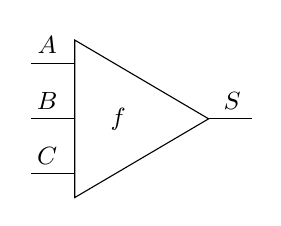
\begin{tikzpicture}[font=\small]
\draw(0,-1)--(0,1)--(1.7,0)--cycle;\node at(.55,0){$f$};
\draw(-.55,.7)--(0,.7);\node[above]at(-.35,.7){$A$};\draw(-.55,0)--(0,0);\node[above]at(-.35,0){$B$};\draw(-.55,-.7)--(0,-.7);\node[above]at(-.35,-.7){$C$};
\draw(1.7,0)--(2.25,0);\node[above]at(2,0){$S$};
\end{tikzpicture}
\end{center}
Mô tả phép hợp thành trong một operad phức tạp hơn đôi chút so với phạm trù vì có nhiều chỉ số biến hơn; tuy nhiên ý tưởng thì đơn giản. Hình~7.4 (trang~\pageref{fig:ctseven-operad-composition}) cho thấy các cấu xạ đang được hợp thành.\ctsevennote{Nguyên bản ghi tham chiếu chưa được giải quyết ``Figure ??''. Hình~7.4 của bản gốc minh họa đúng phép hợp thành đang mô tả, với các đối tượng trung gian $S,T$ biến mất; bản dịch khôi phục tham chiếu đó.} Chú ý rằng $S$ và $T$ biến mất khỏi hợp thành, nhưng điều này tương tự cách đối tượng ở giữa biến mất khỏi phép hợp thành các cấu xạ trong một phạm trù:
\begin{center}
\begin{tikzpicture}[>=Stealth,font=\small]
\node[draw=red,dashed,inner sep=4pt](l)at(0,0){$A\xrightarrow{f}S\xrightarrow{g}X$};
\node[align=center,text width=4.2cm](m)at(4.1,0){các cấu xạ bên trái hợp thành\\để cho ra};
\node[draw=red,dashed,inner sep=4pt](r)at(8,0){$A\xrightarrow{g\circ f}X$};
\end{tikzpicture}
\end{center}
Sau đây là định nghĩa, lấy từ Spivak~[41]. Hãy chuyển đến Ví dụ~7.4.1.3 nếu định nghĩa trở nên quá khó.

\noindent\textbf{Định nghĩa 7.4.1.1.}\keepwithnext
Một \emph{operad $\mathcal O$} được định nghĩa như sau: ta công bố một số thành phần (A. đối tượng, B. cấu xạ, C. các đồng nhất, D. các phép hợp thành) và chứng minh chúng tuân theo một số luật (1. luật đồng nhất, 2. luật kết hợp). Cụ thể, ta công bố
\begin{enumerate}[label=\Alph*.]
\item một lớp $\Ob(\mathcal O)$, mỗi phần tử được gọi là một \emph{đối tượng của $\mathcal O$};
\item với mỗi đối tượng $y\in\Ob(\mathcal O)$, tập hữu hạn $n\in\Ob(\mathbf{Fin})$ và tập các đối tượng có chỉ số trong $n$, $x:n\to\Ob(\mathcal O)$, một tập $\mathcal O_n(x;y)\in\Ob(\Set)$; các phần tử của nó được gọi là \emph{cấu xạ từ $x$ đến $y$ trong $\mathcal O$};
\item với mỗi đối tượng $x\in\Ob(\mathcal O)$, một cấu xạ được chỉ định, ký hiệu $\id_x\in\mathcal O_1(x;x)$ và gọi là \emph{cấu xạ đồng nhất trên $x$}.
\item Cho $s:m\to n$ là một cấu xạ trong $\mathbf{Fin}$. Cho $z\in\Ob(\mathcal O)$ là một đối tượng, $y:n\to\Ob(\mathcal O)$ là một tập các đối tượng có chỉ số trong $n$, và $x:m\to\Ob(\mathcal O)$ là một tập các đối tượng có chỉ số trong $m$. Với mỗi phần tử $i\in n$, viết $m_i:=s^{-1}(i)$ cho nghịch ảnh của $i$ theo $s$, và viết $x_i=x|_{m_i}:m_i\to\Ob(\mathcal O)$ cho hạn chế của $x$ lên $m_i$. Khi ấy ta công bố một hàm
\stepcounter{equation}
\begin{equation}
\circ:\mathcal O_n(y;z)\times\prod_{i\in n}\mathcal O_{m_i}(x_i;y(i))\longrightarrow\mathcal O_m(x;z),
\tag{7.17}
\end{equation}
gọi là \emph{công thức hợp thành}.
\end{enumerate}
% Source: printed p. 454; PDF p. 463
Cho một tập các đối tượng có chỉ số trong $n$, $x:n\to\Ob(\mathcal O)$, và một đối tượng $y\in\Ob(\mathcal O)$, đôi khi ta lạm dụng ký hiệu và ký hiệu tập các cấu xạ từ $x$ đến $y$ bằng $\mathcal O(x_1,\ldots,x_n;y)$.\footnote{Có ba sự lạm dụng ký hiệu khi viết $\mathcal O(x_1,\ldots,x_n;y)$. Thứ nhất, nó lẫn lộn tập $n\in\Ob(\mathbf{Fin})$ với lực lượng $|n|\in\mathbb N$ của tập ấy. Nhưng thay vì viết $\mathcal O(x_1,\ldots,x_{|n|};y)$, sẽ nhất quán hơn nếu viết $\mathcal O(x(1),\ldots,x(|n|);y)$, vì ta đã gán một ý nghĩa khác cho chỉ số dưới ở phần~D. Tuy vậy, ngay cả ký hiệu này cũng ngụ ý không có cơ sở rằng tập $n$ đã được trang bị một thứ tự tuyến tính, trong khi chưa có thứ tự nào như vậy. Có thể xem đây là một sự lạm dụng nghiêm trọng hơn, nhưng xem Nhận xét~7.4.1.2.} Khi thuận tiện, ta có thể viết $\Hom_{\mathcal O}(x_1,\ldots,x_n;y)$ thay cho $\mathcal O(x_1,\ldots,x_n;y)$. Ta có thể ký hiệu một cấu xạ $\varphi\in\mathcal O_n(x;y)$ bằng $\varphi:x\to y$ hoặc $\varphi:(x_1,\ldots,x_n)\to y$; ta nói mỗi $x_i$ là một \emph{đối tượng miền} của $\varphi$, và $y$ là \emph{đối tượng đối miền} của $\varphi$. Ta dùng ký hiệu trung tố cho công thức hợp thành, chẳng hạn $\psi\circ(\varphi_1,\ldots,\varphi_n)$.

Sau đó phải chứng minh các \emph{luật operad} sau đúng:
\begin{enumerate}[label=\arabic*.]
\item Với mọi $x_1,\ldots,x_n,y\in\Ob(\mathcal O)$ và mọi cấu xạ $\varphi:(x_1,\ldots,x_n)\to y$, ta có
\[
\varphi\circ(\id_{x_1},\ldots,\id_{x_n})=\varphi\qquad\text{và}\qquad\id_y\circ\varphi=\varphi.
\]
\item Cho $m\xrightarrow{s}n\xrightarrow{t}p$ là các cấu xạ hợp thành được trong $\mathbf{Fin}$. Cho $z\in\Ob(\mathcal O)$ là một đối tượng; cho $y:p\to\Ob(\mathcal O)$, $x:n\to\Ob(\mathcal O)$ và $w:m\to\Ob(\mathcal O)$ lần lượt là các tập đối tượng có chỉ số trong $p$, trong $n$ và trong $m$. Với mỗi $i\in p$, viết $n_i=t^{-1}(i)$ cho nghịch ảnh, và $x_i:n_i\to\Ob(\mathcal O)$ cho hạn chế. Tương tự, với mỗi $k\in n$, viết $m_k=s^{-1}(k)$ và $w_k:m_k\to\Ob(\mathcal O)$; với mỗi $i\in p$, viết $m_{i,-}=(t\circ s)^{-1}(i)$ và $w_{i,-}:m_{i,-}\to\Ob(\mathcal O)$; với mỗi $j\in n_i$, viết $m_{i,j}:=s^{-1}(j)$ và $w_{i,j}:m_{i,j}\to\Ob(\mathcal O)$. Khi đó sơ đồ sau giao hoán:
\begin{center}
\begin{tikzpicture}[>=Stealth,font=\scriptsize]
\node(t)at(0,0){$\begin{gathered}\mathcal O_p(y;z)\times\prod_{i\in p}\mathcal O_{n_i}(x_i;y(i))\times\\\prod_{i\in p,\ j\in n_i}\mathcal O_{m_{i,j}}(w_{i,j};x_i(j))\end{gathered}$};
\node(l)at(-3,-1.65){$\mathcal O_n(x;z)\times\prod_{k\in n}\mathcal O_{m_k}(w_k;x(k))$};
\node(r)at(3,-1.65){$\mathcal O_p(y;z)\times\prod_{i\in p}\mathcal O_{m_{i,-}}(w_{i,-};y(i))$};
\node(b)at(0,-3){$\mathcal O_m(w;z)$};
\draw[->](t.south west)--(l.north);\draw[->](t.south east)--(r.north);\draw[->](l.south)--(b.north west);\draw[->](r.south)--(b.north east);
\end{tikzpicture}
\end{center}
\end{enumerate}

\noindent\textit{Nhận xét 7.4.1.2.}\keepwithnext
Nhận xét này xét sự lạm dụng ký hiệu trong Định nghĩa~7.4.1.1 và cách nó liên hệ với một tác động của nhóm đối xứng lên mỗi tập cấu xạ trong định nghĩa operad. Ta theo ký hiệu của Định nghĩa~7.4.1.1, nhất là cách dùng chỉ số dưới trong công thức hợp thành.

Giả sử $\mathcal O$ là một operad, $z\in\Ob(\mathcal O)$ là một đối tượng, $y:n\to\Ob(\mathcal O)$ là một tập các đối tượng có chỉ số trong $n$, và $\varphi:y\to z$ là một cấu xạ. Nếu ta đặt một thứ tự tuyến tính trên $n$, cho phép viết $\varphi:(y(1),\ldots,y(|n|))\to z$, thì thay đổi thứ tự tuyến tính tương đương với việc tìm một
